\chapter{Detalles de Implementación y Experimentos}\label{chapter:implementation}

\section{Detalles de implementaci\'on}

En esta secci\'on se abordar\'an algunos detalles que se tuvieron en cuenta a la hora de implementar este m\'odulo.

\subsection{Modelos}

Primeramente obs\'ervese que el rango de niveles de gris de una imagen se define como $[0,M)$. Por ende al transformar la imagen a una funci\'on de tono de gris utilizando la f\'ormula (1.11) cuando el nivel de gris es 0 el tono de gris es $M$, lo cual contradice que el rango de tono de gris para el modelo LIP es $[0,M)$. Por este motivo tanto para la clase \verb|LIPImage| como \verb|LIPSpace| antes de cambiar la imagen de niveles de gris a tonos de gris y viceversa esta primero se procesa de tal forma que el menor valor admisible sea un n\'umero cercano a cero pero mayor que este. En esta implementaci\'on se decidi\'o utilizar el n\'umero $0.0001$. No se opt\'o por otro alternativas como por ejemplo el \'epsilon de la m\'aquina porque al realizar operaciones aritm\'eticas este valor se convert\'ia en cero y por ende no solucionaba el problema planteado. Esta tambi\'en se hizo en la implementaci\'on del modelo PLIP. Para el caso del modelo SLIP no fue necesario pues se utiliza una funci\'on de tono de gris, se trabaja directamente con los niveles de gris.

Otro problema que fue necesario resolver es que en el modelo HLIP los niveles de gris de la imagen a transformar deben estar en el rango $(0,M)$. La soluci\'on propuesta fue hacer algo similar al caso anterior pero solo antes de cambiar la imagen de nivel de gris a tono de gris.

Las implementaciones de todos los modelos tal y como se explic\'o en el cap\'itulo anterior se puede encontrar en el subm\'odulo ``models'', cada uno en su archivo correspondiente.

\subsection{M\'etricas}

Como se explic\'o en el cap\'itulo exterior se implementaron dos m\'etricas: EMEE y $C_p(p)$. La implementaci\'on de estas m\'etricas se puede encontrar en el subm\'odulo ``metrics''. Este subm\'odulo consta de dos archivos: ``emee.py'' y ``contrast\_pixel''. 

En el archivo ``emee.py'' se encuentran dos funciones: \verb|emee| y \verb|find_min_max|. La primera devuelve el valor de EMEE de una imagen dada como entrada. Adem\'as recibe como par\'ametros el valor de $\alpha$, las dimensiones de los bloques en los que se desea dividir la imagen y una constante $c$. Esta constante se utiliza para evitar la divisi\'on por $0$ en (1.33). Se suma tanto al numerador como al denominador de las fracciones que aparecen. La constante que se utiliz\'o para calcular los mejores par\'ametros fue $0.5$. Esto tambi\'en para evitar que una divisi\'on por un n\'umero muy cercano a 0 diera un resultado demasiado grande. La funci\'on \verb|find_min_max| se utiliza para calcular el menor y mayor valor de intensidad de un bloque. Da como salida una tupla con dicho valores en ese orden y recibe una imagen y 4 enteros: $n_1,n_2,m_1,m_2$, tal que $(n_1,m_1)$ son las coordenadas donde inicia el bloque y; $n_2$ y $m_2$ son la dimensi\'on horizontal y vertical del bloque respectivamente.

En el archivo ``contrast\_pixel.py'' se encuentra tres funciones. La primera funci\'on \verb|abs_contrast_2_pixels| se utiliza para calcular el contraste absoluto entre 2 pixeles. Recibe dos tuplas de 3 elementos, tal que cada una representa representa un pixel (las coordenadas y el valor de intensidad del pixel), y el valor de $M$.  La segunda funci\'on \verb|contras_pixel| calcula el contraste de un pixel en una imagen; recibe como par\'ametros una tupla que representa al pixel, la imagen, el valor de $M$ y un valor $v$ que indica el radio de la vecindad a considerarse. La \'ultima funci\'on \verb|contrast_img| da como salida el contraste promedio de un pixel en una imagen, o sea $C_p$. Esta funci\'on recibe como par\'ametros la imagen, el valor de $M$ y el radio de la vecindad que se debe tener en cuenta alrededor de un pixel. Como calcular el contraste para cada pixel de una imagen es un proceso que puede demorar seg\'un el tama\~no de la imagen, se tom\'o la decisi\'on de, para imagen cuya resoluci\'on fuese mayor que $300\times300$, escoger un subconjunto de pixeles. El criterio para escoger dichos pixeles fue el siguiente:

\begin{enumerate}
	\item Iniciar desde la posici\'on $(0,0)$
	\item Si se analiz\'o el pixel en la posici\'on $(i,j)$ el pr\'oximo pixel a analizar es el pixel $(i,j+3)$
	\item Una vez terminada de analizar una fila $i$ la pr\'oxima fila a analizar es la fila $i+3$.
\end{enumerate}

El radio de la vecindad que se tom\'o para calcular el contraste de cada pixel fue de 2. Al comparar ambas formas se pudo comprobar que, para im\'agenes con una resoluci\'on grande, la forma propuesta, reduce considerablemente el tiempo de ejecuci\'on, afectando en una cantidad despreciable el resultado final.

\subsection{Algoritmos}

La implementaci\'on de los algoritmos explicados en el cap\'itulo anterior se encuentra en el subm\'odulo ``algorithms''. Este subm\'odulo consta de dos archivos: ``affine\_transform.py'' y ``lee.py''. 

El archivo ``affine\_transform.py'' contiene dos funciones \verb|affine_transform| y \verb|space_affine_transform|. La primera da como salida la transformaci\'on af\'in explicada en el cap\'itulo anterior utilizando las operaciones aritm\'eticas lineales. Recibe como par\'ametros una imagen y los extremos del intervalo en el cual se va a realizar la transformaci\'on. La segunda funci\'on da como salida la transformaci\'on af\'in utilizando las operaciones aritm\'eticas de un modelo espec\'ifico. Adem\'as de recibir los mismos par\'ametros que la funci\'on, recibe una instancia de tipo \verb|LogSpace|. Este par\'ametro se utiliza para indicar con que modelo se quiere realizar la transformaci\'on. Los extremos del intervalo de entrada deben ser los del modelo utilizado para obtener los mejores resultados.

El archivo ``lee.py'' tambi\'en contiene dos funciones \verb|lee| y \verb|space_lee|. La primera es el Algoritmo de Lee cl\'asico. Recibe como par\'ametros una imagen, un entero $n$ (dimensi\'on de la ventana) y los valores de $theta,~\rho$ y $\zeta$, dando como salida la imagen procesada por este algoritmo con dichos par\'ametros. La segunda funci\'on es el Algoritmo de Lee extendido para utilizarse con cualquiera de los modelos. Recibe como par\'ametros una imagen, los valores de $n,~\eta,~\sigma,~\delta$ y una instancia de tipo \verb|LogSpace|. Este \'ultimo indica con que modelo se deben realizar las operaciones aritm\'eticas para este algoritmo.

\section{Experimentos}
Para los experimentos que a continuaci\'on se muestran se utilizaron im\'agenes en escala de gris de 8 bits, o sea que los valores de intensidades de los pixeles eran n\'umeros enteros en el intervalo $[0,255]$.  

\subsection{Curvas de los isomorfismos}
Lo primero que se muestra son las curvas de los diferentes isomorfismos, iniciando por los no parametrizados que se muestran en la Fig 3.1. Para los isomorfismos LIP y PSLIP se muestra adem\'as los puntos respectivos a los valores: 0 (rojo), 128 (naranja) y 255(amarillo). Para el caso de HLIP se muestran los puntos para los valores: 1 (rojo), 128 (naranja) y 255 (amarillo). Para el caso del modelo SLIP se muestran los puntos para los valores: -255 (morado) -128(verde) 0 (rojo), 128 (naranja) y 255(amarillo).

\begin{figure}
	\begin{center}
		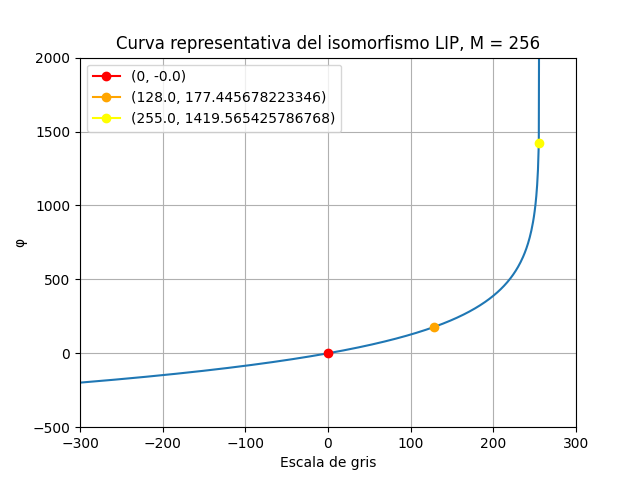
\includegraphics[width=5.5 cm]{images/clasics_curves/lip_curve.png}
		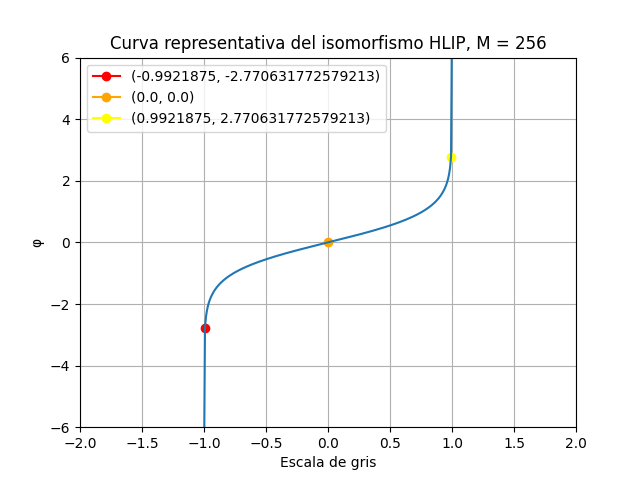
\includegraphics[width=5.5 cm]{images/clasics_curves/hlip_curve.png}
		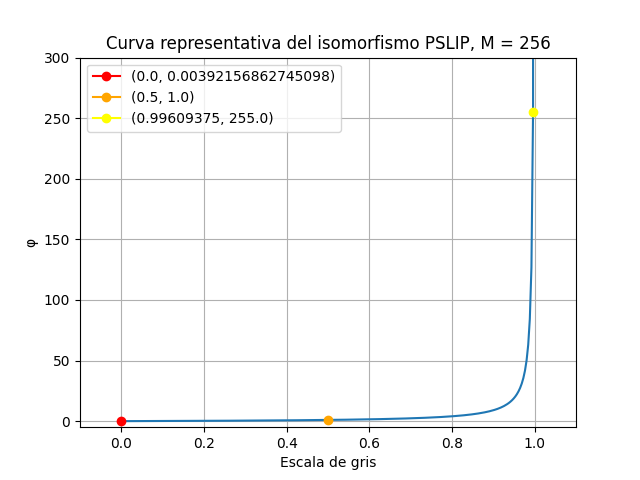
\includegraphics[width=5.5 cm]{images/clasics_curves/pslip_curve.png}
		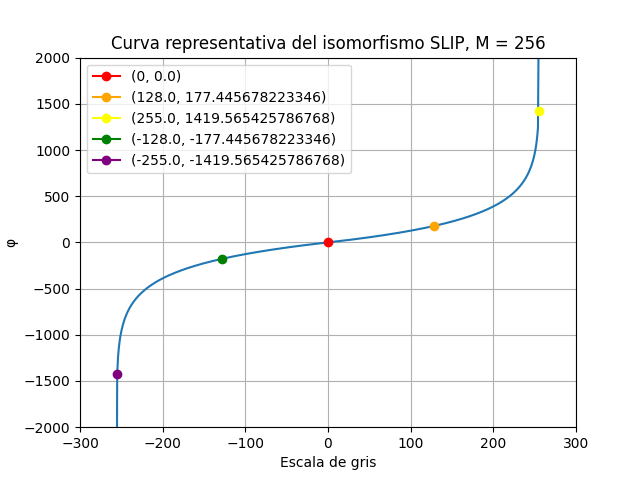
\includegraphics[width=5.5 cm]{images/clasics_curves/slip_curve.png}
		\caption{Curvas representativas de los modelos no parametrizados}
	\end{center}
\end{figure}

En las Fig 3.2 y Fig 3.3 se pueden observar varias curvas del modelo PLIP y PPSLIP utilizando diferentes valores de $\lambda(M)$. En ambos modelos se puede apreciar la tendencia a la linealidad a medida que el valor de $\lambda(M)$ aumenta. Obse\'ervese que los puntos correspondiente a 0 (rojo), 128 (naranja) y 255 (amarillo) se van acercando a una l\'inea recta. Tambi\'en se muestra que los nuevos valores que aparecen siguen manteniendo la estructura logar\'itmica.

\begin{figure}
	\begin{center}
		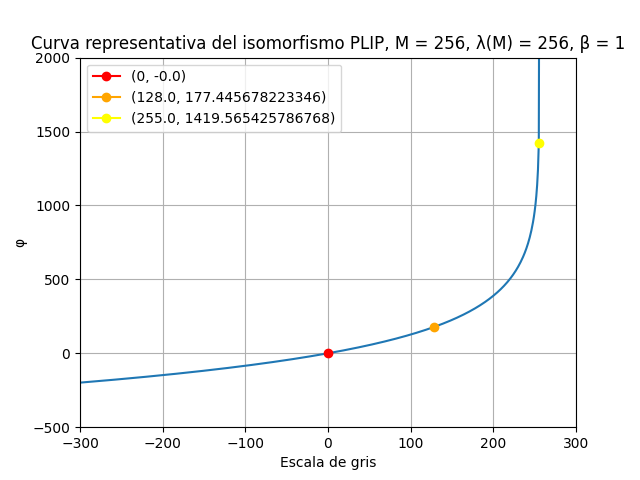
\includegraphics[width=5.5 cm]{images/plip_curves/plip_curve_256.png}
		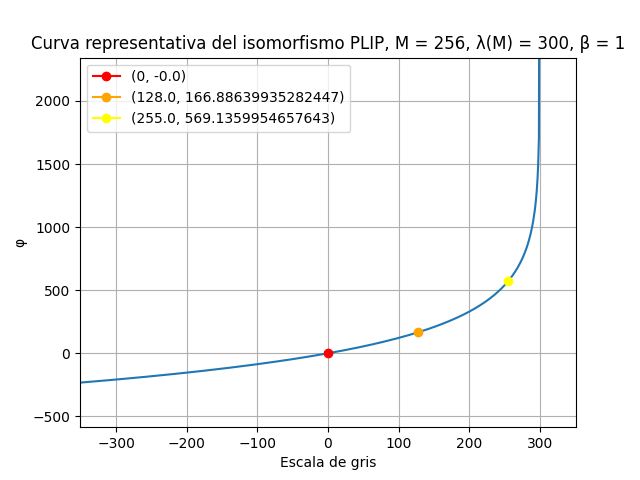
\includegraphics[width=5.5 cm]{images/plip_curves/plip_curve_300.png}
		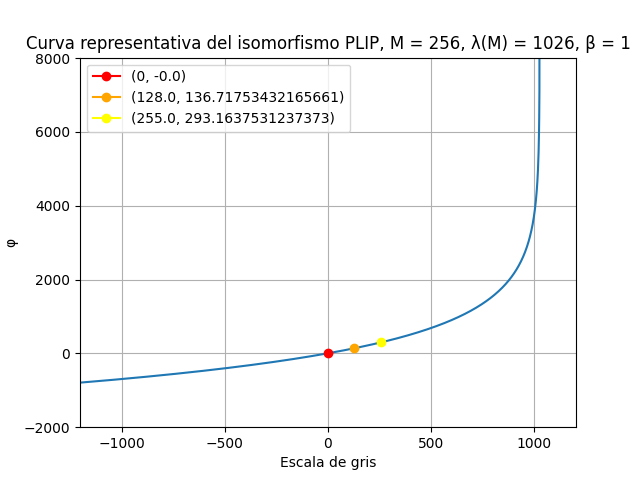
\includegraphics[width=5.5 cm]{images/plip_curves/plip_curve_1026.png}
		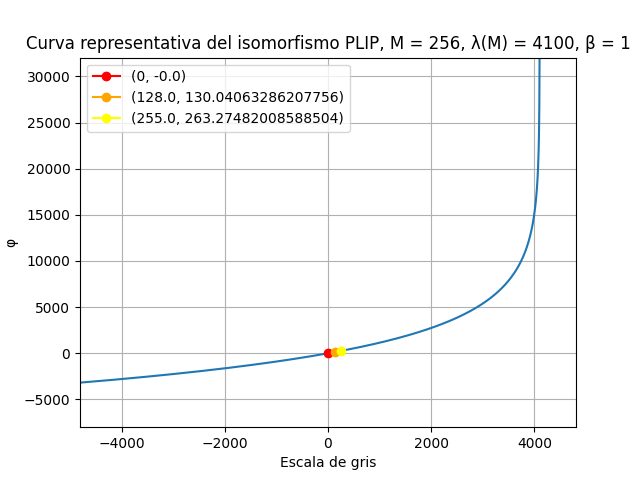
\includegraphics[width=5.5 cm]{images/plip_curves/plip_curve_4100.png}
		\caption{Curvas representativas del modelo PLIP con diferentes valores de $\lambda(M)$}
	\end{center}
\end{figure}

\begin{figure}
	\begin{center}
		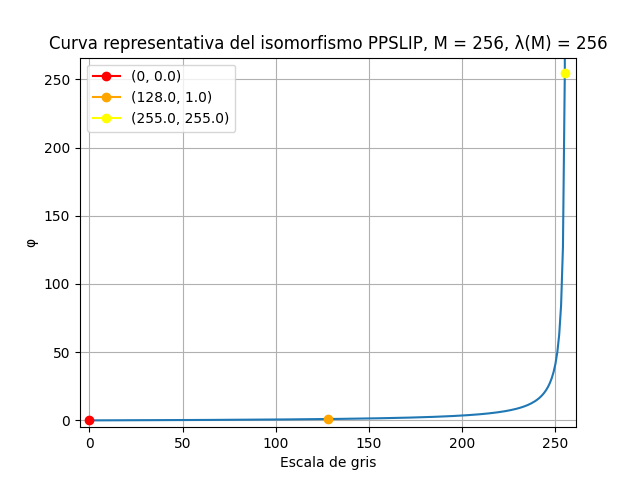
\includegraphics[width=5.0 cm]{images/ppslip_curves/ppslip_curve_256.png}
		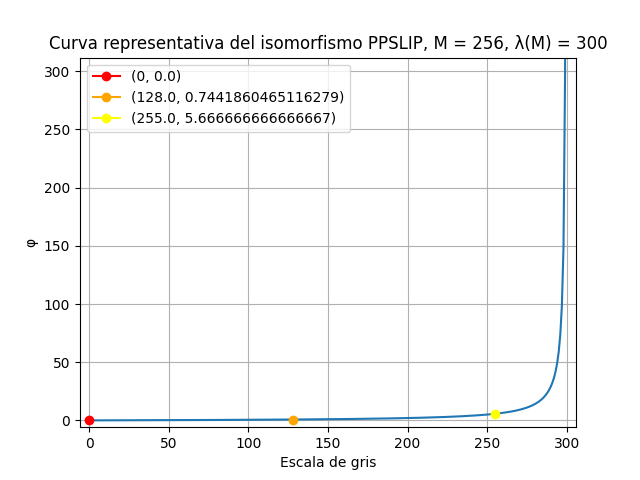
\includegraphics[width=5.0 cm]{images/ppslip_curves/ppslip_curve_300.png}
		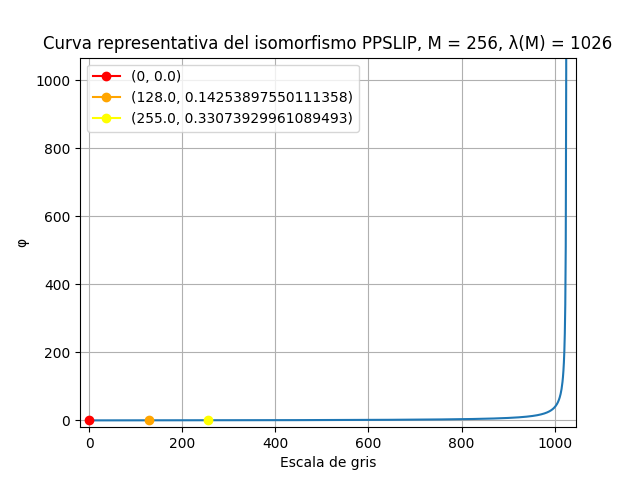
\includegraphics[width=5.0 cm]{images/ppslip_curves/ppslip_curve_1026.png}
		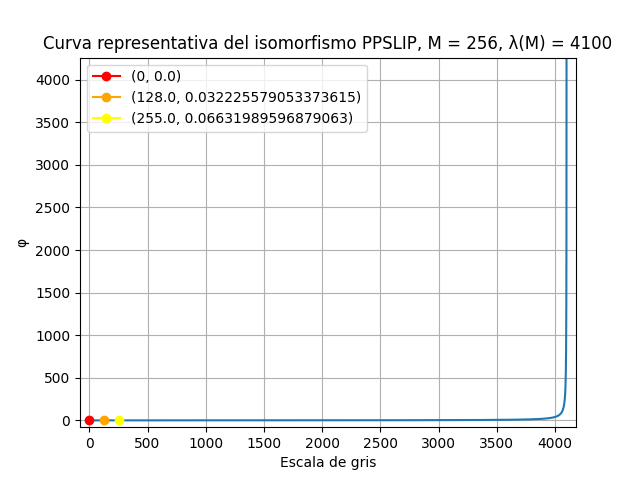
\includegraphics[width=5.0 cm]{images/ppslip_curves/ppslip_curve_4100.png}
		\caption{Curvas representativas del modelo PPSLIP con diferentes valores de $\lambda(M)$}
	\end{center}
\end{figure}

\section{Suma de im\'agenes}